\subsection{Gateway}
	Un \textit{gateway} è una componente localizzata all'interno di un'azienda che permette di rendere uniforme l'interfaccia di accesso ai dati dei singoli dispositivi configurati all'interno del gateway stesso.
	\newline
	Dai gateway è possibile inoltre configurare funzioni di accumulo dei pacchetti contenenti i dati dei sensori o di impostare alcuni timer, al termine dei quali deve essere effettuato l'invio dei dati all'interno dei rispettivi topic di Kafka.
	\newline
	Tutte le configurazioni vengono ricevute tramite appositi topic adibiti esclusivamente a questa funzione.
	\begin{itemize}
		\item La componente è stata sviluppata in Java 11.
	\end{itemize}
	
	\subsubsection{Diagramma dei package}%%%%%%%%%%%%OK
	  	\begin{figure}[H]
			\centering
			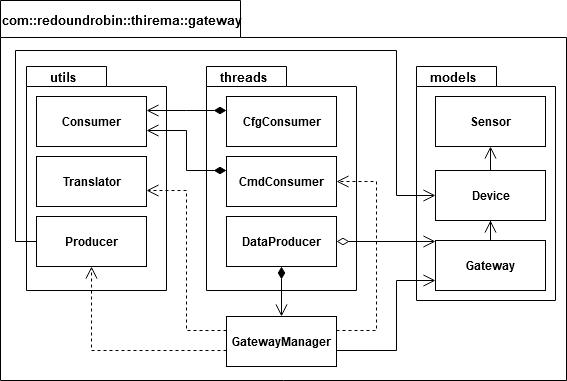
\includegraphics[scale=0.550]{res/images/GATEWAY/GatewayPackage.png}
			\caption{Diagramma dei package per la componente gateway}
			\label{Diagramma 1}
		\end{figure}
	\subsubsection{Dipendenze esterne}	
		La componente gateway ha due dipendenze esterne: 
			\begin{itemize}
				\item \textbf{KafkaProducer<K, V>}, classe concreta che implementa l'interfaccia Producer<K,V>. Svolge il compito di client per il cluster kafka, pubblicando dati all'interno di un topic. La classe Producer ne possiede un riferimento.
				\item \textbf{KafkaConsumer<K,V>}, classe concreta che implementa l'interfaccia Consumer<K,V>. Svolge il compito di client per il cluster Kafka, consumando i messaggi resenti all'interno di uno o più topic. La classe Consumer ne possiede un riferimento.
			\end{itemize}	
		\newpage		

	\begin{landscape}
		\subsubsection{Diagramma delle classi}%%%%%%%%%%%%%%%%%%%%%%%OK
		  	\begin{figure}[H]
				\centering
				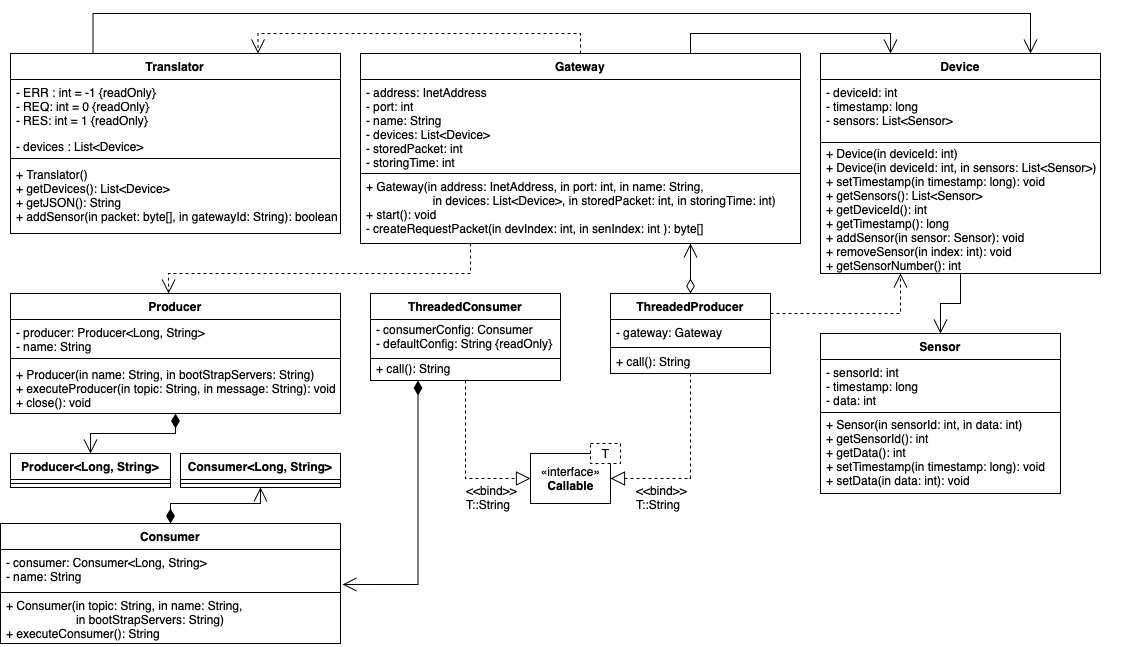
\includegraphics[scale=0.499]{res/images/GATEWAY/ClassiGateway.png}
				\caption{Diagramma delle classi per la componente gateway}
				\label{Diagramma 2}
			\end{figure}
	Come si evince dal diagramma la classe ThreadedConsumer contiene un Consumer per poter reperire da un topic Kafka le configurazioni per il gateway. Il ThreadedProducer invece contiene un riferimento a Gateway, in cui si trova la business logic per la richiesta al simulatore e l'invio dei dati a Kafka. Per poter far ciò necessita della classe translator per convertire i dati in JSON e delle classi Device e Sensor per costruire la lista di dispositivi a cui dovrà richiedere i dati.
	\end{landscape}
		
	\begin{landscape}
		\subsubsection{Diagramma di sequenza}%%%%%%%%%%%%%%%%%%%%%%%OK
		  	\begin{figure}[H]
				\centering
				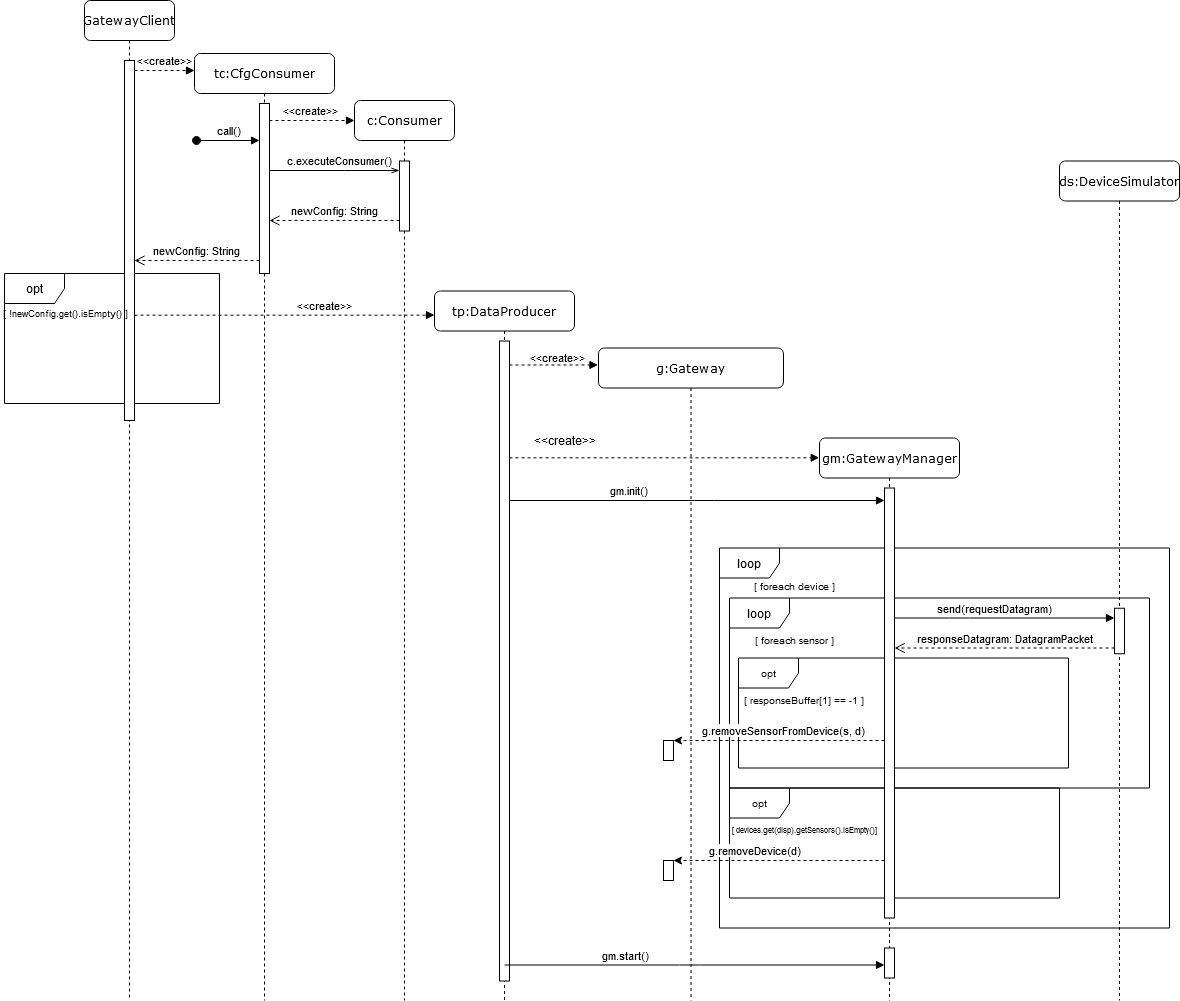
\includegraphics[scale=0.400]{res/images/GATEWAY/RichiestaInvioGateway.png}
				\caption{Diagramma di sequenza che rappresenta la richiesta di una prima configurazione ed un primo settaggio del gateway}
				\label{Diagramma 3}
			\end{figure}
			Nel diagramma di sequenza è rappresentata la richiesta e la ricezione di una prima configurazione da parte del ThreadedConsumer. La configurazione viene quindi passata al ThreadedProducer, che tramite un metodo crea il Gateway (sulla base della configurazione ottenuta) e questo, tramite il metodo init() verifica che tutti i dispositivi nella configurazione siano effettivamente presenti.
	\end{landscape}
	
	\subsubsection{Diagramma di attività}%%%%%%%%%%%%%%OK
		\begin{figure}[H]
			\centering
			\includegraphics[scale=0.500]{res/images/GATEWAY/gateway.start().png}
			\caption{Diagramma di attività che rappresenta un'iterazione all'interno del metodo start() della classe gateway}
			\label{Diagramma 4}
		\end{figure}
		 Nel diagramma è rappresentato il metodo start() della classe Gateway, in cui vengono creati dei pacchetti di richiesta e vengono inviati al simulatore dei dispositivi. Quest'ultimo, dopo aver generato i dati, invia un pacchetto di risposta che, se è integro, viene aggiunto ad un buffer che, una volta pieno, viene inviato ad un topic Kafka.   
		